% Options for packages loaded elsewhere
\PassOptionsToPackage{unicode}{hyperref}
\PassOptionsToPackage{hyphens}{url}
%
\documentclass[
]{article}
\usepackage{amsmath,amssymb}
\usepackage{lmodern}
\usepackage{iftex}
\ifPDFTeX
  \usepackage[T1]{fontenc}
  \usepackage[utf8]{inputenc}
  \usepackage{textcomp} % provide euro and other symbols
\else % if luatex or xetex
  \usepackage{unicode-math}
  \defaultfontfeatures{Scale=MatchLowercase}
  \defaultfontfeatures[\rmfamily]{Ligatures=TeX,Scale=1}
\fi
% Use upquote if available, for straight quotes in verbatim environments
\IfFileExists{upquote.sty}{\usepackage{upquote}}{}
\IfFileExists{microtype.sty}{% use microtype if available
  \usepackage[]{microtype}
  \UseMicrotypeSet[protrusion]{basicmath} % disable protrusion for tt fonts
}{}
\makeatletter
\@ifundefined{KOMAClassName}{% if non-KOMA class
  \IfFileExists{parskip.sty}{%
    \usepackage{parskip}
  }{% else
    \setlength{\parindent}{0pt}
    \setlength{\parskip}{6pt plus 2pt minus 1pt}}
}{% if KOMA class
  \KOMAoptions{parskip=half}}
\makeatother
\usepackage{xcolor}
\usepackage[margin=1in]{geometry}
\usepackage{color}
\usepackage{fancyvrb}
\newcommand{\VerbBar}{|}
\newcommand{\VERB}{\Verb[commandchars=\\\{\}]}
\DefineVerbatimEnvironment{Highlighting}{Verbatim}{commandchars=\\\{\}}
% Add ',fontsize=\small' for more characters per line
\usepackage{framed}
\definecolor{shadecolor}{RGB}{248,248,248}
\newenvironment{Shaded}{\begin{snugshade}}{\end{snugshade}}
\newcommand{\AlertTok}[1]{\textcolor[rgb]{0.94,0.16,0.16}{#1}}
\newcommand{\AnnotationTok}[1]{\textcolor[rgb]{0.56,0.35,0.01}{\textbf{\textit{#1}}}}
\newcommand{\AttributeTok}[1]{\textcolor[rgb]{0.77,0.63,0.00}{#1}}
\newcommand{\BaseNTok}[1]{\textcolor[rgb]{0.00,0.00,0.81}{#1}}
\newcommand{\BuiltInTok}[1]{#1}
\newcommand{\CharTok}[1]{\textcolor[rgb]{0.31,0.60,0.02}{#1}}
\newcommand{\CommentTok}[1]{\textcolor[rgb]{0.56,0.35,0.01}{\textit{#1}}}
\newcommand{\CommentVarTok}[1]{\textcolor[rgb]{0.56,0.35,0.01}{\textbf{\textit{#1}}}}
\newcommand{\ConstantTok}[1]{\textcolor[rgb]{0.00,0.00,0.00}{#1}}
\newcommand{\ControlFlowTok}[1]{\textcolor[rgb]{0.13,0.29,0.53}{\textbf{#1}}}
\newcommand{\DataTypeTok}[1]{\textcolor[rgb]{0.13,0.29,0.53}{#1}}
\newcommand{\DecValTok}[1]{\textcolor[rgb]{0.00,0.00,0.81}{#1}}
\newcommand{\DocumentationTok}[1]{\textcolor[rgb]{0.56,0.35,0.01}{\textbf{\textit{#1}}}}
\newcommand{\ErrorTok}[1]{\textcolor[rgb]{0.64,0.00,0.00}{\textbf{#1}}}
\newcommand{\ExtensionTok}[1]{#1}
\newcommand{\FloatTok}[1]{\textcolor[rgb]{0.00,0.00,0.81}{#1}}
\newcommand{\FunctionTok}[1]{\textcolor[rgb]{0.00,0.00,0.00}{#1}}
\newcommand{\ImportTok}[1]{#1}
\newcommand{\InformationTok}[1]{\textcolor[rgb]{0.56,0.35,0.01}{\textbf{\textit{#1}}}}
\newcommand{\KeywordTok}[1]{\textcolor[rgb]{0.13,0.29,0.53}{\textbf{#1}}}
\newcommand{\NormalTok}[1]{#1}
\newcommand{\OperatorTok}[1]{\textcolor[rgb]{0.81,0.36,0.00}{\textbf{#1}}}
\newcommand{\OtherTok}[1]{\textcolor[rgb]{0.56,0.35,0.01}{#1}}
\newcommand{\PreprocessorTok}[1]{\textcolor[rgb]{0.56,0.35,0.01}{\textit{#1}}}
\newcommand{\RegionMarkerTok}[1]{#1}
\newcommand{\SpecialCharTok}[1]{\textcolor[rgb]{0.00,0.00,0.00}{#1}}
\newcommand{\SpecialStringTok}[1]{\textcolor[rgb]{0.31,0.60,0.02}{#1}}
\newcommand{\StringTok}[1]{\textcolor[rgb]{0.31,0.60,0.02}{#1}}
\newcommand{\VariableTok}[1]{\textcolor[rgb]{0.00,0.00,0.00}{#1}}
\newcommand{\VerbatimStringTok}[1]{\textcolor[rgb]{0.31,0.60,0.02}{#1}}
\newcommand{\WarningTok}[1]{\textcolor[rgb]{0.56,0.35,0.01}{\textbf{\textit{#1}}}}
\usepackage{graphicx}
\makeatletter
\def\maxwidth{\ifdim\Gin@nat@width>\linewidth\linewidth\else\Gin@nat@width\fi}
\def\maxheight{\ifdim\Gin@nat@height>\textheight\textheight\else\Gin@nat@height\fi}
\makeatother
% Scale images if necessary, so that they will not overflow the page
% margins by default, and it is still possible to overwrite the defaults
% using explicit options in \includegraphics[width, height, ...]{}
\setkeys{Gin}{width=\maxwidth,height=\maxheight,keepaspectratio}
% Set default figure placement to htbp
\makeatletter
\def\fps@figure{htbp}
\makeatother
\setlength{\emergencystretch}{3em} % prevent overfull lines
\providecommand{\tightlist}{%
  \setlength{\itemsep}{0pt}\setlength{\parskip}{0pt}}
\setcounter{secnumdepth}{-\maxdimen} % remove section numbering
\usepackage{xeCJK}
\ifLuaTeX
  \usepackage{selnolig}  % disable illegal ligatures
\fi
\IfFileExists{bookmark.sty}{\usepackage{bookmark}}{\usepackage{hyperref}}
\IfFileExists{xurl.sty}{\usepackage{xurl}}{} % add URL line breaks if available
\urlstyle{same} % disable monospaced font for URLs
\hypersetup{
  hidelinks,
  pdfcreator={LaTeX via pandoc}}

\author{}
\date{\vspace{-2.5em}}

\begin{document}

\hypertarget{biostatistics-homework-6}{%
\section{Biostatistics Homework 6}\label{biostatistics-homework-6}}

By \(\mathbb{L}\)umi (张鹿鸣12112618)

\vspace{5mm}

\hypertarget{gas-mileage}{%
\subsection{1. Gas Mileage}\label{gas-mileage}}

1.1) C

1.2) B

\hypertarget{old-and-new-machines}{%
\subsection{2. Old and New Machines}\label{old-and-new-machines}}

2.1)

\(H_0\) : The new machine is not faster than the old machine on average
(\(\mu_\text{new} \geq \mu_\text{old}\)).

\(H_1\) : The new machine is faster than the old machine on average
(\(\mu_\text{new} < \mu_\text{old}\)).

2.2)

It means that there is a 0.05 chance to reject the null hypothesis when
the null hypothesis is true.

2.3)

The q2\_table.txt:

Oldmachine 42.7 43.8 42.5 43.1 44.0 43.6 43.3 43.5 41.7 44.1

Newmachine 42.1 41.3 42.4 43.2 41.8 41.0 41.8 42.8 42.3 42.7

\begin{Shaded}
\begin{Highlighting}[]
\NormalTok{machines }\OtherTok{\textless{}{-}} \FunctionTok{as.data.frame}\NormalTok{(}\FunctionTok{t}\NormalTok{(}\FunctionTok{read.table}\NormalTok{(}\StringTok{\textquotesingle{}q2\_table.txt\textquotesingle{}}\NormalTok{, }\AttributeTok{sep =} \StringTok{\textquotesingle{}}\SpecialCharTok{\textbackslash{}t}\StringTok{\textquotesingle{}}\NormalTok{, }\AttributeTok{row.names =} \DecValTok{1}\NormalTok{)))}
\NormalTok{mean\_old }\OtherTok{\textless{}{-}} \FunctionTok{mean}\NormalTok{(machines}\SpecialCharTok{$}\NormalTok{Oldmachine)}
\NormalTok{mean\_new }\OtherTok{\textless{}{-}} \FunctionTok{mean}\NormalTok{(machines}\SpecialCharTok{$}\NormalTok{Newmachine)}
\NormalTok{var\_old }\OtherTok{\textless{}{-}} \FunctionTok{var}\NormalTok{(machines}\SpecialCharTok{$}\NormalTok{Oldmachine)}
\NormalTok{var\_new }\OtherTok{\textless{}{-}} \FunctionTok{var}\NormalTok{(machines}\SpecialCharTok{$}\NormalTok{Newmachine)}
\NormalTok{statistics }\OtherTok{\textless{}{-}} \FunctionTok{data.frame}\NormalTok{(}
  \AttributeTok{mean =} \FunctionTok{c}\NormalTok{(mean\_old, mean\_new),}
  \AttributeTok{variance =} \FunctionTok{c}\NormalTok{(var\_old, var\_new)}
\NormalTok{)}
\FunctionTok{rownames}\NormalTok{(statistics) }\OtherTok{\textless{}{-}} \FunctionTok{c}\NormalTok{(}\StringTok{\textquotesingle{}Old\textquotesingle{}}\NormalTok{, }\StringTok{\textquotesingle{}New\textquotesingle{}}\NormalTok{)}
\NormalTok{statistics}
\end{Highlighting}
\end{Shaded}

\begin{verbatim}
##      mean  variance
## Old 43.23 0.5623333
## New 42.14 0.4671111
\end{verbatim}

So the statistics are:

\[
\bar{x}_\text{new} = 42.14 , s_\text{new}^2 \approx 0.5623
\]

\[
\bar{x}_\text{old} = 43.23 , s_\text{old}^2 \approx 0.4671 
\]

2.4)

We should use an independent two sample T-test. Since we have
independent samples that are not paired.

We should check our samples are randomly and independently selected.

It is also important that the samples follow T-distributions. Or that
the population follows a normal distribution.

\begin{Shaded}
\begin{Highlighting}[]
\FunctionTok{boxplot}\NormalTok{(machines)}
\end{Highlighting}
\end{Shaded}

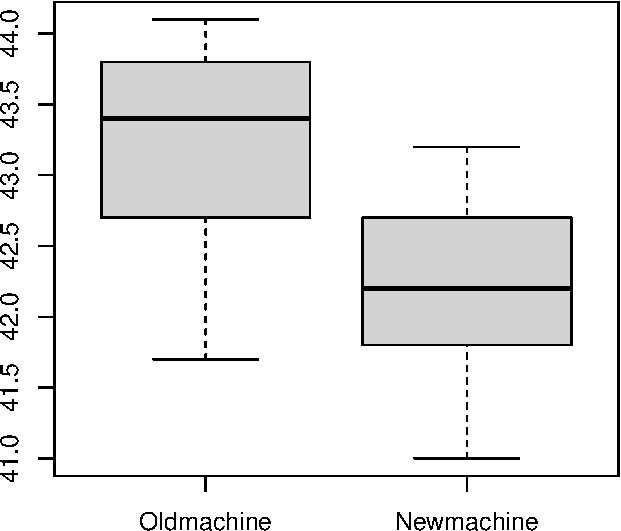
\includegraphics{Homework6_files/figure-latex/unnamed-chunk-2-1.pdf}

From the plot, I think we can say that our sample roughly follows a
T-distribution, so using a T-test is reasonable.

We should also make sure that the variance between the two samples don't
vary too much. In our samples, it doesn't.

2.5)

So the common variance is :

\[
s^2 = \frac{(n_\text{new} - 1) s_\text{new}^2 + (n_\text{old} - 1) s_\text{old}^2}{n_\text{new} + n_\text{old} - 2} = \frac{9 \times 0.5623 + 9 \times 0.4671}{18} = 0.5147
\]

The T-score is:

\[
t = \frac{\bar{x}_\text{new} - \bar{x}_\text{old}}{\sqrt{s^2(\frac{1}{n_\text{new}} + \frac{1}{n_\text{old}})}} = \frac{42.14 - 43.23}{\sqrt{0.5147 \times(\frac{1}{10} + \frac{1}{10})}} \approx -3.397
\]

The p-value is:

\begin{Shaded}
\begin{Highlighting}[]
\FunctionTok{pt}\NormalTok{(}\SpecialCharTok{{-}}\FloatTok{3.397}\NormalTok{, }\DecValTok{18}\NormalTok{)}
\end{Highlighting}
\end{Shaded}

\begin{verbatim}
## [1] 0.001606392
\end{verbatim}

\begin{Shaded}
\begin{Highlighting}[]
\FunctionTok{t.test}\NormalTok{(machines}\SpecialCharTok{$}\NormalTok{Newmachine, machines}\SpecialCharTok{$}\NormalTok{Oldmachine, }\AttributeTok{alternative =} \StringTok{"less"}\NormalTok{)}
\end{Highlighting}
\end{Shaded}

\begin{verbatim}
## 
##  Welch Two Sample t-test
## 
## data:  machines$Newmachine and machines$Oldmachine
## t = -3.3972, df = 17.847, p-value = 0.001621
## alternative hypothesis: true difference in means is less than 0
## 95 percent confidence interval:
##        -Inf -0.5333684
## sample estimates:
## mean of x mean of y 
##     42.14     43.23
\end{verbatim}

From the \texttt{t.test()} function in R, we can see that our answers
are quite right.

2.6)

D

(I don't know if B is correct or not, we reject the null hypothesis if
the significance level is 0.05, but it doesn't mean the null hypothesis
is wrong.)

\hypertarget{anova}{%
\subsection{3. ANOVA}\label{anova}}

C

\hypertarget{another-anova}{%
\subsection{4. Another ANOVA}\label{another-anova}}

B

(Since the variance of the data is mainly contributed by the variance
within the groups (MSW).)

\hypertarget{another-anova-1}{%
\subsection{5. Another ANOVA}\label{another-anova-1}}

C

\hypertarget{anova-and-t-test}{%
\subsection{6. ANOVA and T-test}\label{anova-and-t-test}}

B

(Using multiple T-tests increase the chance of making a Type I error in
your study, I don't think it is very good to say that it increases the
probability of making a type I error)

\hypertarget{post-hoc-anova}{%
\subsection{\texorpdfstring{7. \textbf{post-hoc}
ANOVA}{7. post-hoc ANOVA}}\label{post-hoc-anova}}

A (or between multiple groups)

\hypertarget{fisheries}{%
\subsection{8. Fisheries}\label{fisheries}}

8.1)

\(H_0\): The mean weights of fish caught from the three lakes are not
different.

\(H_1\): The mean weights of fish caught from the three lakes are
different.

8.2)

\begin{Shaded}
\begin{Highlighting}[]
\NormalTok{anova }\OtherTok{\textless{}{-}} \FunctionTok{data.frame}\NormalTok{(}\AttributeTok{d.f. =} \FunctionTok{c}\NormalTok{(}\DecValTok{2}\NormalTok{,}\DecValTok{9}\NormalTok{,}\DecValTok{11}\NormalTok{),}
                    \AttributeTok{SS =} \FunctionTok{c}\NormalTok{(}\FloatTok{17.04}\NormalTok{, }\FloatTok{14.19}\NormalTok{, }\FloatTok{31.23}\NormalTok{),}
                    \AttributeTok{MS =} \FunctionTok{c}\NormalTok{(}\FloatTok{17.04}\SpecialCharTok{/}\DecValTok{2}\NormalTok{, }\FloatTok{14.19}\SpecialCharTok{/}\DecValTok{9}\NormalTok{, }\ConstantTok{NA}\NormalTok{))}
\FunctionTok{row.names}\NormalTok{(anova) }\OtherTok{\textless{}{-}} \FunctionTok{c}\NormalTok{(}\StringTok{"Between"}\NormalTok{, }\StringTok{"Within"}\NormalTok{, }\StringTok{"Total"}\NormalTok{)}
\NormalTok{anova}
\end{Highlighting}
\end{Shaded}

\begin{verbatim}
##         d.f.    SS       MS
## Between    2 17.04 8.520000
## Within     9 14.19 1.576667
## Total     11 31.23       NA
\end{verbatim}

So the F-score is:

\[
F = \frac{\text{MSB}}{\text{MSW}} = 8.52 \div 1.5767 = 5.404
\]

So the p-value is:

\begin{Shaded}
\begin{Highlighting}[]
\FunctionTok{pf}\NormalTok{(}\FloatTok{5.404}\NormalTok{, }\DecValTok{2}\NormalTok{, }\DecValTok{9}\NormalTok{, }\AttributeTok{lower.tail =}\NormalTok{ F)}
\end{Highlighting}
\end{Shaded}

\begin{verbatim}
## [1] 0.0287282
\end{verbatim}

8.3)

The p-value is 0.0287, so we should reject the null hypothesis.

\hypertarget{tar-in-cigarettes}{%
\subsection{9. Tar in Cigarettes}\label{tar-in-cigarettes}}

\begin{Shaded}
\begin{Highlighting}[]
\NormalTok{tar }\OtherTok{\textless{}{-}} \FunctionTok{data.frame}\NormalTok{(}
  \AttributeTok{BrandA =} \FunctionTok{c}\NormalTok{(}\FloatTok{10.21}\NormalTok{,}\FloatTok{10.25}\NormalTok{,}\FloatTok{10.24}\NormalTok{,}\FloatTok{9.80}\NormalTok{,}\FloatTok{9.77}\NormalTok{,}\FloatTok{9.73}\NormalTok{),}
  \AttributeTok{BrandB =} \FunctionTok{c}\NormalTok{(}\FloatTok{11.32}\NormalTok{,}\FloatTok{11.20}\NormalTok{,}\FloatTok{11.40}\NormalTok{,}\FloatTok{10.50}\NormalTok{,}\FloatTok{10.68}\NormalTok{,}\FloatTok{10.90}\NormalTok{),}
  \AttributeTok{BrandC =} \FunctionTok{c}\NormalTok{(}\FloatTok{11.60}\NormalTok{,}\FloatTok{11.90}\NormalTok{,}\FloatTok{11.80}\NormalTok{,}\FloatTok{12.30}\NormalTok{,}\FloatTok{12.20}\NormalTok{,}\FloatTok{12.20}\NormalTok{)}
\NormalTok{)}
\end{Highlighting}
\end{Shaded}

9.1)

\(H_0\): The tar contents for the three different brands of cigarettes
are not different.

\(H_1\): The tar contents for the three different brands of cigarettes
are different.

9.2)

\begin{Shaded}
\begin{Highlighting}[]
\CommentTok{\# We need to melt the data to perform anova test}
\FunctionTok{library}\NormalTok{(reshape2)}
\NormalTok{molten\_tar }\OtherTok{\textless{}{-}} \FunctionTok{melt}\NormalTok{(tar)}
\end{Highlighting}
\end{Shaded}

\begin{verbatim}
## No id variables; using all as measure variables
\end{verbatim}

\begin{Shaded}
\begin{Highlighting}[]
\NormalTok{res }\OtherTok{\textless{}{-}} \FunctionTok{aov}\NormalTok{(value}\SpecialCharTok{\textasciitilde{}}\NormalTok{variable, }\AttributeTok{data =}\NormalTok{ molten\_tar)}
\FunctionTok{summary}\NormalTok{(res)}
\end{Highlighting}
\end{Shaded}

\begin{verbatim}
##             Df Sum Sq Mean Sq F value   Pr(>F)    
## variable     2 12.000   6.000   65.46 3.89e-08 ***
## Residuals   15  1.375   0.092                     
## ---
## Signif. codes:  0 '***' 0.001 '**' 0.01 '*' 0.05 '.' 0.1 ' ' 1
\end{verbatim}

We can see from the result summary that we have a F-value of 65.46 and a
p-value of \(3.98\times 10^{-8}\). Thus we should reject the null
hypothesis.

9.3)

\begin{Shaded}
\begin{Highlighting}[]
\NormalTok{mean\_a }\OtherTok{\textless{}{-}} \FunctionTok{mean}\NormalTok{(tar}\SpecialCharTok{$}\NormalTok{BrandA)}
\NormalTok{mean\_b }\OtherTok{\textless{}{-}} \FunctionTok{mean}\NormalTok{(tar}\SpecialCharTok{$}\NormalTok{BrandB)}
\NormalTok{mean\_c }\OtherTok{\textless{}{-}} \FunctionTok{mean}\NormalTok{(tar}\SpecialCharTok{$}\NormalTok{BrandC)}
\NormalTok{s2\_a }\OtherTok{\textless{}{-}} \FunctionTok{var}\NormalTok{(tar}\SpecialCharTok{$}\NormalTok{BrandA)}
\NormalTok{s2\_b }\OtherTok{\textless{}{-}} \FunctionTok{var}\NormalTok{(tar}\SpecialCharTok{$}\NormalTok{BrandB)}
\NormalTok{s2\_c }\OtherTok{\textless{}{-}} \FunctionTok{var}\NormalTok{(tar}\SpecialCharTok{$}\NormalTok{BrandC)}
\NormalTok{s2\_ab }\OtherTok{\textless{}{-}}\NormalTok{ (}\DecValTok{5} \SpecialCharTok{*}\NormalTok{ s2\_a }\SpecialCharTok{+} \DecValTok{5} \SpecialCharTok{*}\NormalTok{ s2\_b)}\SpecialCharTok{/}\DecValTok{10}
\NormalTok{s2\_ac }\OtherTok{\textless{}{-}}\NormalTok{ (}\DecValTok{5} \SpecialCharTok{*}\NormalTok{ s2\_a }\SpecialCharTok{+} \DecValTok{5} \SpecialCharTok{*}\NormalTok{ s2\_c)}\SpecialCharTok{/}\DecValTok{10}
\NormalTok{s2\_bc }\OtherTok{\textless{}{-}}\NormalTok{ (}\DecValTok{5} \SpecialCharTok{*}\NormalTok{ s2\_b }\SpecialCharTok{+} \DecValTok{5} \SpecialCharTok{*}\NormalTok{ s2\_c)}\SpecialCharTok{/}\DecValTok{10}
\NormalTok{t\_ab }\OtherTok{\textless{}{-}}\NormalTok{ (mean\_a }\SpecialCharTok{{-}}\NormalTok{ mean\_b)}\SpecialCharTok{/}\FunctionTok{sqrt}\NormalTok{(s2\_ab }\SpecialCharTok{*}\NormalTok{ (}\DecValTok{1}\SpecialCharTok{/}\DecValTok{6} \SpecialCharTok{+} \DecValTok{1}\SpecialCharTok{/}\DecValTok{6}\NormalTok{))}
\NormalTok{t\_ac }\OtherTok{\textless{}{-}}\NormalTok{ (mean\_a }\SpecialCharTok{{-}}\NormalTok{ mean\_c)}\SpecialCharTok{/}\FunctionTok{sqrt}\NormalTok{(s2\_ac }\SpecialCharTok{*}\NormalTok{ (}\DecValTok{1}\SpecialCharTok{/}\DecValTok{6} \SpecialCharTok{+} \DecValTok{1}\SpecialCharTok{/}\DecValTok{6}\NormalTok{))}
\NormalTok{t\_bc }\OtherTok{\textless{}{-}}\NormalTok{ (mean\_b }\SpecialCharTok{{-}}\NormalTok{ mean\_c)}\SpecialCharTok{/}\FunctionTok{sqrt}\NormalTok{(s2\_bc }\SpecialCharTok{*}\NormalTok{ (}\DecValTok{1}\SpecialCharTok{/}\DecValTok{6} \SpecialCharTok{+} \DecValTok{1}\SpecialCharTok{/}\DecValTok{6}\NormalTok{))}
\FunctionTok{c}\NormalTok{(t\_ab, t\_ac, t\_bc)}
\end{Highlighting}
\end{Shaded}

\begin{verbatim}
## [1]  -5.491522 -13.000542  -5.358510
\end{verbatim}

I just realized after I did this that the Fisher's Least Significant
Difference requires to use MSW as the common variant. No matter, we show
here that the resulting t-score using MSW and standard deviation between
two samples are different.

\begin{Shaded}
\begin{Highlighting}[]
\NormalTok{t\_ab\_msw }\OtherTok{\textless{}{-}}\NormalTok{ (mean\_a }\SpecialCharTok{{-}}\NormalTok{ mean\_b)}\SpecialCharTok{/}\FunctionTok{sqrt}\NormalTok{(}\FloatTok{0.092} \SpecialCharTok{*}\NormalTok{ (}\DecValTok{1}\SpecialCharTok{/}\DecValTok{6} \SpecialCharTok{+} \DecValTok{1}\SpecialCharTok{/}\DecValTok{6}\NormalTok{))}
\NormalTok{t\_ac\_msw }\OtherTok{\textless{}{-}}\NormalTok{ (mean\_a }\SpecialCharTok{{-}}\NormalTok{ mean\_c)}\SpecialCharTok{/}\FunctionTok{sqrt}\NormalTok{(}\FloatTok{0.092} \SpecialCharTok{*}\NormalTok{ (}\DecValTok{1}\SpecialCharTok{/}\DecValTok{6} \SpecialCharTok{+} \DecValTok{1}\SpecialCharTok{/}\DecValTok{6}\NormalTok{))}
\NormalTok{t\_bc\_msw }\OtherTok{\textless{}{-}}\NormalTok{ (mean\_b }\SpecialCharTok{{-}}\NormalTok{ mean\_c)}\SpecialCharTok{/}\FunctionTok{sqrt}\NormalTok{(}\FloatTok{0.092} \SpecialCharTok{*}\NormalTok{ (}\DecValTok{1}\SpecialCharTok{/}\DecValTok{6} \SpecialCharTok{+} \DecValTok{1}\SpecialCharTok{/}\DecValTok{6}\NormalTok{))}
\FunctionTok{c}\NormalTok{(t\_ab\_msw, t\_ac\_msw, t\_bc\_msw)}
\end{Highlighting}
\end{Shaded}

\begin{verbatim}
## [1]  -5.710402 -11.420805  -5.710402
\end{verbatim}

\begin{Shaded}
\begin{Highlighting}[]
\NormalTok{table }\OtherTok{\textless{}{-}} \FunctionTok{data.frame}\NormalTok{(}
  \AttributeTok{Comparison =} \FunctionTok{c}\NormalTok{(}\StringTok{"A vs. B"}\NormalTok{, }\StringTok{"A vs. C"}\NormalTok{, }\StringTok{"B vs. C"}\NormalTok{),}
  \AttributeTok{t\_score =} \FunctionTok{c}\NormalTok{(t\_ab, t\_ac, t\_bc),}
  \AttributeTok{p\_value =} \FunctionTok{c}\NormalTok{(}\FunctionTok{pt}\NormalTok{(t\_ab, }\DecValTok{15}\NormalTok{) }\SpecialCharTok{*} \DecValTok{2}\NormalTok{, }\FunctionTok{pt}\NormalTok{(t\_ac, }\DecValTok{15}\NormalTok{) }\SpecialCharTok{*} \DecValTok{2}\NormalTok{, }\FunctionTok{pt}\NormalTok{(t\_bc, }\DecValTok{15}\NormalTok{) }\SpecialCharTok{*} \DecValTok{2}\NormalTok{),}
  \AttributeTok{t\_score\_msw =} \FunctionTok{c}\NormalTok{(t\_ab\_msw, t\_ac\_msw, t\_bc\_msw),}
  \AttributeTok{p\_value\_msw =} \FunctionTok{c}\NormalTok{(}\FunctionTok{pt}\NormalTok{(t\_ab\_msw, }\DecValTok{15}\NormalTok{) }\SpecialCharTok{*} \DecValTok{2}\NormalTok{, }\FunctionTok{pt}\NormalTok{(t\_ac\_msw, }\DecValTok{15}\NormalTok{) }\SpecialCharTok{*} \DecValTok{2}\NormalTok{, }\FunctionTok{pt}\NormalTok{(t\_bc\_msw, }\DecValTok{15}\NormalTok{) }\SpecialCharTok{*} \DecValTok{2}\NormalTok{),}
  \AttributeTok{p\_adj =} \FunctionTok{c}\NormalTok{(}\FunctionTok{pt}\NormalTok{(t\_ab\_msw, }\DecValTok{15}\NormalTok{) }\SpecialCharTok{*} \DecValTok{2}\NormalTok{, }\FunctionTok{pt}\NormalTok{(t\_ac\_msw, }\DecValTok{15}\NormalTok{) }\SpecialCharTok{*} \DecValTok{2}\NormalTok{, }\FunctionTok{pt}\NormalTok{(t\_bc\_msw, }\DecValTok{15}\NormalTok{) }\SpecialCharTok{*} \DecValTok{2}\NormalTok{) }\SpecialCharTok{*} \FunctionTok{choose}\NormalTok{(}\DecValTok{3}\NormalTok{, }\DecValTok{2}\NormalTok{)}
\NormalTok{)}
\NormalTok{table}
\end{Highlighting}
\end{Shaded}

\begin{verbatim}
##   Comparison    t_score      p_value t_score_msw  p_value_msw        p_adj
## 1    A vs. B  -5.491522 6.203182e-05   -5.710402 4.128135e-05 1.238440e-04
## 2    A vs. C -13.000542 1.436101e-09  -11.420805 8.473751e-09 2.542125e-08
## 3    B vs. C  -5.358510 7.969684e-05   -5.710402 4.128135e-05 1.238440e-04
\end{verbatim}

Thus the table should be:

\begin{Shaded}
\begin{Highlighting}[]
\NormalTok{table[, }\FunctionTok{c}\NormalTok{(}\DecValTok{1}\NormalTok{,}\DecValTok{4}\NormalTok{,}\DecValTok{5}\NormalTok{,}\DecValTok{6}\NormalTok{)]}
\end{Highlighting}
\end{Shaded}

\begin{verbatim}
##   Comparison t_score_msw  p_value_msw        p_adj
## 1    A vs. B   -5.710402 4.128135e-05 1.238440e-04
## 2    A vs. C  -11.420805 8.473751e-09 2.542125e-08
## 3    B vs. C   -5.710402 4.128135e-05 1.238440e-04
\end{verbatim}

\begin{Shaded}
\begin{Highlighting}[]
\CommentTok{\# Trying to write a all{-}in{-}one function to calculate the pairwise t{-}tests}
\NormalTok{get\_msw }\OtherTok{\textless{}{-}} \ControlFlowTok{function}\NormalTok{(data)\{}
\NormalTok{  msw }\OtherTok{\textless{}{-}} \DecValTok{0}
  \ControlFlowTok{for}\NormalTok{(i }\ControlFlowTok{in} \DecValTok{1} \SpecialCharTok{:} \FunctionTok{dim}\NormalTok{(data)[}\DecValTok{2}\NormalTok{])\{}
\NormalTok{    msw }\OtherTok{\textless{}{-}}\NormalTok{ msw }\SpecialCharTok{+}\NormalTok{ (}\FunctionTok{length}\NormalTok{(data[,i]) }\SpecialCharTok{{-}} \DecValTok{1}\NormalTok{) }\SpecialCharTok{*} \FunctionTok{var}\NormalTok{(data[,i])}
\NormalTok{  \}}
  \FunctionTok{return}\NormalTok{(msw }\SpecialCharTok{/}\NormalTok{ (}\FunctionTok{dim}\NormalTok{(data)[}\DecValTok{1}\NormalTok{] }\SpecialCharTok{*} \FunctionTok{dim}\NormalTok{(data)[}\DecValTok{2}\NormalTok{] }\SpecialCharTok{{-}} \FunctionTok{dim}\NormalTok{(data)[}\DecValTok{2}\NormalTok{]))}
\NormalTok{\}}

\NormalTok{pairwise\_t }\OtherTok{\textless{}{-}} \ControlFlowTok{function}\NormalTok{(data)\{}
\NormalTok{  msw }\OtherTok{\textless{}{-}} \FunctionTok{get\_msw}\NormalTok{(data)}
\NormalTok{  row\_names }\OtherTok{\textless{}{-}} \FunctionTok{c}\NormalTok{()}
\NormalTok{  t\_score }\OtherTok{\textless{}{-}} \FunctionTok{c}\NormalTok{()}
\NormalTok{  p\_value }\OtherTok{\textless{}{-}} \FunctionTok{c}\NormalTok{()}
  
  \ControlFlowTok{for}\NormalTok{(i }\ControlFlowTok{in} \DecValTok{1} \SpecialCharTok{:}\NormalTok{ (}\FunctionTok{dim}\NormalTok{(data)[}\DecValTok{2}\NormalTok{] }\SpecialCharTok{{-}} \DecValTok{1}\NormalTok{))\{}
    \ControlFlowTok{for}\NormalTok{(j }\ControlFlowTok{in}\NormalTok{ (i }\SpecialCharTok{+} \DecValTok{1}\NormalTok{) }\SpecialCharTok{:} \FunctionTok{dim}\NormalTok{(data)[}\DecValTok{2}\NormalTok{])\{}
\NormalTok{      a }\OtherTok{\textless{}{-}}\NormalTok{ data[,i]}
\NormalTok{      b }\OtherTok{\textless{}{-}}\NormalTok{ data[,j]}
      
      \CommentTok{\# Add two column names to the row name}
\NormalTok{      row\_names }\OtherTok{\textless{}{-}} \FunctionTok{append}\NormalTok{(row\_names,}\FunctionTok{paste0}\NormalTok{(}\FunctionTok{colnames}\NormalTok{(data)[i], }\StringTok{" vs. "}\NormalTok{, }\FunctionTok{colnames}\NormalTok{(data)[j]))}
      
      \CommentTok{\# Calculate the t\_score}
\NormalTok{      t }\OtherTok{\textless{}{-}}\NormalTok{ (}\FunctionTok{mean}\NormalTok{(a) }\SpecialCharTok{{-}} \FunctionTok{mean}\NormalTok{(b)) }\SpecialCharTok{/} \FunctionTok{sqrt}\NormalTok{(msw }\SpecialCharTok{*}\NormalTok{ (}\DecValTok{1} \SpecialCharTok{/} \FunctionTok{length}\NormalTok{(a) }\SpecialCharTok{+} \DecValTok{1} \SpecialCharTok{/} \FunctionTok{length}\NormalTok{(b)))}
\NormalTok{      t\_score }\OtherTok{\textless{}{-}} \FunctionTok{append}\NormalTok{(t\_score, t)}
      
      \CommentTok{\# Calculate the p\_value}
\NormalTok{      p\_value }\OtherTok{\textless{}{-}} \FunctionTok{append}\NormalTok{(p\_value, }\FunctionTok{pt}\NormalTok{(t, }\FunctionTok{dim}\NormalTok{(data)[}\DecValTok{1}\NormalTok{] }\SpecialCharTok{*} \FunctionTok{dim}\NormalTok{(data)[}\DecValTok{2}\NormalTok{] }\SpecialCharTok{{-}} \FunctionTok{dim}\NormalTok{(data)[}\DecValTok{2}\NormalTok{]) }\SpecialCharTok{*} \DecValTok{2}\NormalTok{)}
\NormalTok{    \}}
\NormalTok{  \}}
\NormalTok{  table }\OtherTok{\textless{}{-}} \FunctionTok{data.frame}\NormalTok{(}
    \AttributeTok{Comparison =}\NormalTok{ row\_names,}
    \AttributeTok{t =}\NormalTok{ t\_score,}
    \AttributeTok{p =}\NormalTok{ p\_value,}
    \AttributeTok{p.adj =}\NormalTok{ p\_value }\SpecialCharTok{*} \FunctionTok{choose}\NormalTok{(}\FunctionTok{dim}\NormalTok{(data)[}\DecValTok{2}\NormalTok{], }\DecValTok{2}\NormalTok{)}
\NormalTok{  )}
  \FunctionTok{return}\NormalTok{(table)}
\NormalTok{\}}
\FunctionTok{pairwise\_t}\NormalTok{(tar)}
\end{Highlighting}
\end{Shaded}

\begin{verbatim}
##          Comparison          t            p        p.adj
## 1 BrandA vs. BrandB  -5.721192 4.046768e-05 1.214030e-04
## 2 BrandA vs. BrandC -11.442383 8.259836e-09 2.477951e-08
## 3 BrandB vs. BrandC  -5.721192 4.046768e-05 1.214030e-04
\end{verbatim}

Which give identical results, Hooray!

\end{document}
